% File: client_server.tex
% Created: 2015-01-22
% Author: Tesser Paolo
% Email: p.tesser921@gmail.com
% 
%
% Modification History
% Version	Modifier Date	Author			Change
% ====================================================================
% 0.0.1		2015-01-22		Tesser Paolo	inserita sezione capitolo
% ====================================================================
%

\section{Logica di comunicazione client-server} % (fold)
\label{sec:logica_di_comunicazione_client_server}
Per la comunicazione tra i diversi client e il server il programma adotta la libreria RMI che offre un livello di astrazione più elevato rispetto al meccanismo di comunicazione tramite socket. \\
Il suo scopo è quello di rendere trasparenti al programmatore quasi tutti i dettagli della comunicazione su rete. \\
Per implementare il meccanismo offerto da RMI, ci serviamo del package \textbf{objrem} citato nella sezione precedente e dei main delle classi \textbf{PuzzleSolverClient} e \textbf{PuzzleSolverServer}. \\
La logica di comunicazione viene descritta separando la parte del client da quella del server, indicando per ciascuno degli attori le azioni che andranno a compiere. \\ \\

\textbf{Main Thread Server}:
	\begin{enumerate}
		\item crea un oggetto del tipo \textbf{ObjRemImpl}; 
		\item pubblicizza l'oggetto appena creato sul server che ha il nome del parametro passato in input durante l'avvio del programma; 
		\item stampa la conferma che è pronto e si mette in attesa che qualche client effettui delle chiamate sull'oggetto remoto condiviso.
	\end{enumerate}
	\noindent

\textbf{Main Client} (presente un unico flusso):
		\begin{enumerate}
			\item crea un riferimento all'oggetto remoto pubblicizzato dal server, andandolo a prendere grazie al nome del server passato come uno dei tre parametri in input durante l'avvio del programma;
			\item trasforma il file passato come primo parametro in un ArrayList di stringhe;
			\item ricava un identificativo univoco dal server attraverso la chiamata del metodo \textbf{getNewIdPuzzle()} sul riferimento dell'oggetto remoto creato in precedenza;
			\item attraverso l'invocazione del metodo \textbf{setClientPuzzle()} sul riferimento, imposta il sul server il puzzle che vuole andare a risolvere e lo associa al suo identificativo;
			\item sempre attraverso il riferimento chiama il metodo \textbf{solve()} per risolvere il puzzle passato in precedenza;
			\item chiama il metodo \textbf{convert()}, che esegue la conversione solo quando il metodo \textbf{solve()} ha terminato;
			\item preleva il puzzle nel formato che gli serve e lo ottiene in locale dalla chiamata del metodo \textbf{getOutput()} sul riferimento all'oggetto remoto, il quale ritorna un ArrayList<String> che è \textbf{Serializable} di default;
			\item scrive il contenuto precedentemente ottenuto dal server sul file di output passato come secondo parametro durante l'avvio del programma.
		\end{enumerate}
		\noindent
\textbf{Nota}: i metodi che vengono chiamati dal punto 2 a 7 vengono lanciati dal main del client, ma generano l'avvio di un thread sul server, non in conflitto però con il main thread dello stesso server. \\ \\

Per cercare di mantenere un livello di concorrenza tra i diversi client sul server, vengono utilizzate altre due classi che estendo \textbf{Thread} e che vengono, concretizzate e avviate, nei metodi di \textbf{ObjRemImpl}. \\
\textbf{SolveThread Server}:
	\begin{enumerate}
		\item \textbf{Creato e avviato dal}: metodo \textbf{solve()};
		\item \textbf{Avviato quando}: viene chiamato il metodo;
		\item \textbf{Scopo}: risolvere il puzzle passato come parametro al thread.
	\end{enumerate}
	\noindent
	
\textbf{ConcreteThread Server}:
	\begin{enumerate}
		\item \textbf{Creato e avviato dal}: metodo \textbf{concrete()};
		\item \textbf{Avviato quando}: il thread del tipo SolveThread, del client che richiede la conversione, ha terminato l'esecuzione;
		\item \textbf{Scopo}: convertire il puzzle nel formato che servirà al client per la scrittura sul file di output.
	\end{enumerate}
	\noindent
\textbf{Note}: il numero di thread che viene avviato dipenderà da quanti client si connetteranno per risolvere il loro puzzle. \\
Si poteva implementare diversamente, magari attraverso un Thread Pool, ma non essendo richiesto dalla specifica si è deciso di limitarsi ad una cosa più semplice. \\
Inoltre potevano essere implementati anche dei metodi per fare un po' di pulizia sulle HashMap varie, quando il client ha terminato la sua esecuzione.

	\begin{comment}
		\begin{figure}[htbp]
			\centering
			\centerline{n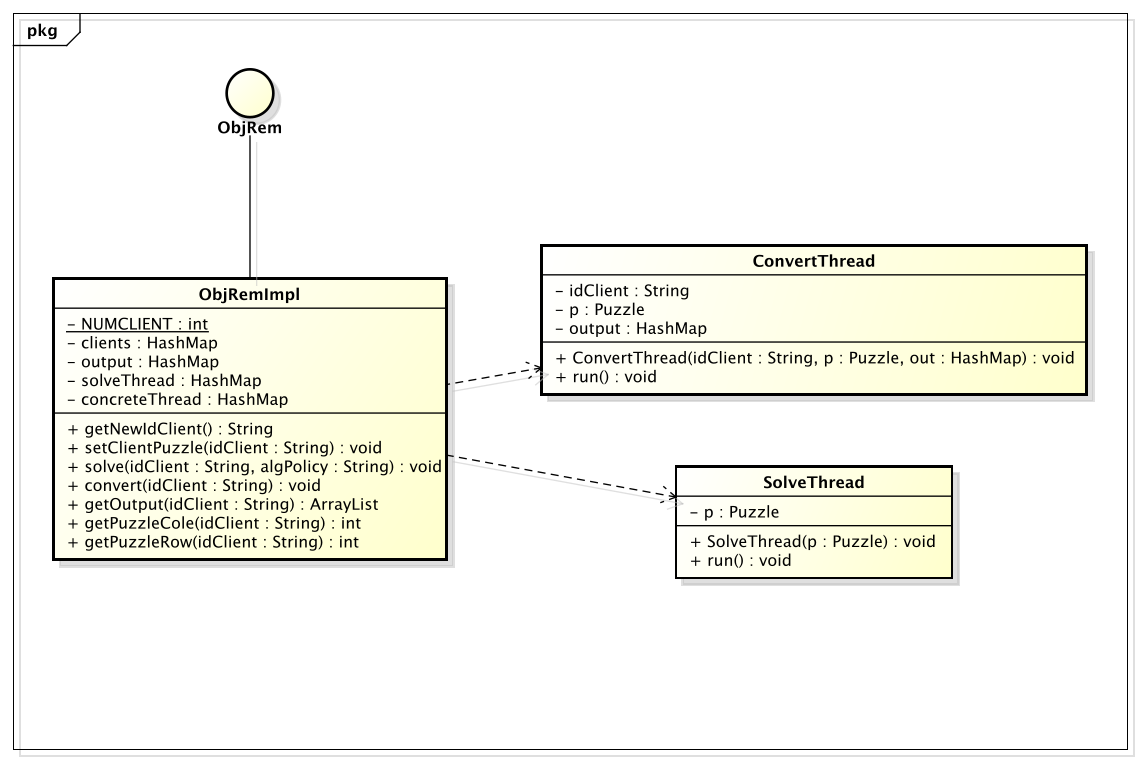
\includegraphics[scale=0.5]{img/objrem.pdf}}
			\caption{Diagramma di sequenza - Relazione Client, Server, ObjRem, SolveThread, ConcreteThread}
			\label{fig:dia_seq_rel_client_server}
		\end{figure}	
	\end{comment}	

% section logica_di_comunicazione_client_server (end)



